\documentclass[11pt]{article}
\usepackage[margin=1in]{geometry}
\usepackage{amsmath,amssymb}
\usepackage{graphicx}
\usepackage{tikz}
\usetikzlibrary{calc,patterns,arrows.meta}
\usepackage[colorlinks=true,linkcolor=blue,citecolor=blue,urlcolor=blue]{hyperref}
\hypersetup{
  pdftitle={Electromagnetic Helix Reactor (EHR): A Multi-Physics Plasma Control Architecture for Advanced Plasma Processing},
  pdfauthor={Zachary Auerbach}
}

\title{Electromagnetic Helix Reactor (EHR): \\ A Multi-Physics Plasma Control Architecture for Advanced Plasma Processing}
\author{Zachary Auerbach}
\date{July 15, 2026}

\begin{document}
\maketitle

\begin{abstract}
This paper proposes the Electromagnetic Helix Reactor (EHR), a multi-physics plasma source architecture that integrates a tunable helical magnetic field, helicon-wave excitation with resonance-matched coupling, and acoustic standing-wave modulation of the neutral gas. The design aims to provide new degrees of spatial control in low-temperature plasmas relevant to semiconductor processing. The baseline operating regime is the magnetized-electron, unmagnetized-ion regime characteristic of helicon sources. Four falsifiable experimental predictions are outlined to test the core elements of the proposed architecture.
\end{abstract}

\section{Introduction}

Low-temperature plasmas are fundamental to semiconductor manufacturing, thin-film deposition, and surface modification. Conventional sources such as inductively coupled plasmas (ICP) and electron cyclotron resonance (ECR) sources typically operate with fixed magnetic geometries and single-mode excitation \cite{lieberman,chabert,oehrlein2018,asmussen1989}. Helicon sources have demonstrated high efficiency through whistler-wave coupling \cite{boswell1984,chen2015}, while acoustic radiation forces are well established for structuring fluids and dusty plasmas \cite{gorkov1962,bruus2012}.

The EHR integrates three elements into a single architecture:
\begin{itemize}
    \item A divergence-free helical magnetic field whose pitch can be tuned via coil currents,
    \item Helicon-mode wave drive with resonance-matched power coupling, and
    \item Acoustic standing-wave modulation of the neutral gas as an independent mesoscale control channel.
\end{itemize}

The central motivation is to move beyond fixed-geometry sources toward a reactor in which key control variables — field-line pitch and acoustic mode structure — can be adjusted in a physically consistent manner. This paper outlines the underlying physical principles, defines a consistent operating regime, and proposes a clear experimental validation path.

\section{System Architecture}

The EHR consists of a cylindrical vacuum chamber, a multi-coil electromagnet producing a helical static field, an RF antenna for $m=1$ helicon excitation, wall-mounted piezoelectric acoustic transducers, and an electrostatic wafer chuck with independent RF bias (Fig.~\ref{fig:tool}).

\begin{figure}[htbp]
\centering
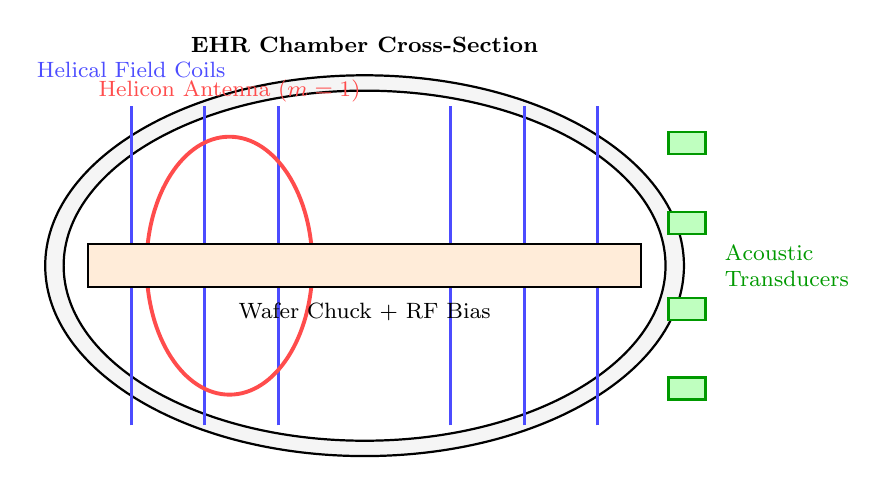
\begin{tikzpicture}[
    scale=0.78,
    every node/.style={font=\footnotesize},
    thick
]
\draw[fill=gray!8, draw=black] (0,0) ellipse (5.2 and 3.1);
\draw[fill=white, draw=black] (0,0) ellipse (4.9 and 2.85);

\foreach \x in {-3.8, -2.6, -1.4, 1.4, 2.6, 3.8} {
    \draw[blue!70, line width=1.1pt] (\x, -2.6) -- (\x, 2.6);
}
\node[blue!70, above] at (-3.8, 2.9) {Helical Field Coils};

\draw[red!70, line width=1.4pt] (-2.2,0) ellipse (1.35 and 2.1);
\node[red!70, above] at (-2.2, 2.5) {Helicon Antenna ($m=1$)};

\draw[fill=orange!15, draw=black, line width=0.9pt] (-4.5,-0.35) rectangle (4.5,0.35);
\node at (0, -0.75) {Wafer Chuck + RF Bias};

\foreach \y in {-2.0, -0.7, 0.7, 2.0} {
    \draw[green!60!black, fill=green!25, line width=0.8pt]
        (4.95, \y-0.18) rectangle (5.55, \y+0.18);
}
\node[green!60!black, right, align=left] at (5.7, 0) {Acoustic\\Transducers};

\node at (0, 3.6) {\textbf{EHR Chamber Cross-Section}};
\end{tikzpicture}
\caption{Schematic cross-section of the proposed EHR showing the helical field coils, helicon antenna, acoustic transducers, and wafer stage.}
\label{fig:tool}
\end{figure}

\section{Electromagnetic Field Architecture}

The static magnetic field combines axial and azimuthal components in cylindrical coordinates:
\begin{equation}
\mathbf{B}(r) = B_z(r)\,\hat{\mathbf{z}} + B_\theta(r)\,\hat{\boldsymbol{\theta}}, \quad B_r = 0.
\label{eq:bfield}
\end{equation}

The local field-line pitch is given by
\begin{equation}
L_p(r) = \frac{2\pi r\, B_z(r)}{B_\theta(r)}.
\label{eq:pitch}
\end{equation}

This pitch constitutes a programmable control variable. A force-free realization is provided by the constant-$\alpha$ Beltrami field \cite{freidberg}:
\begin{equation}
B_z(r) = B_0 J_0(\alpha r), \quad B_\theta(r) = B_0 J_1(\alpha r).
\label{eq:forcefree}
\end{equation}

The dynamic electromagnetic drive is realized through a helicon $m=1$ mode (Fig.~\ref{fig:fieldlines}):
\begin{equation}
\tilde{\mathbf{B}}(r,\theta,z,t) \propto f(r)\exp[i(\theta + kz - \omega t)].
\label{eq:helicon}
\end{equation}

\begin{figure}[htbp]
\centering
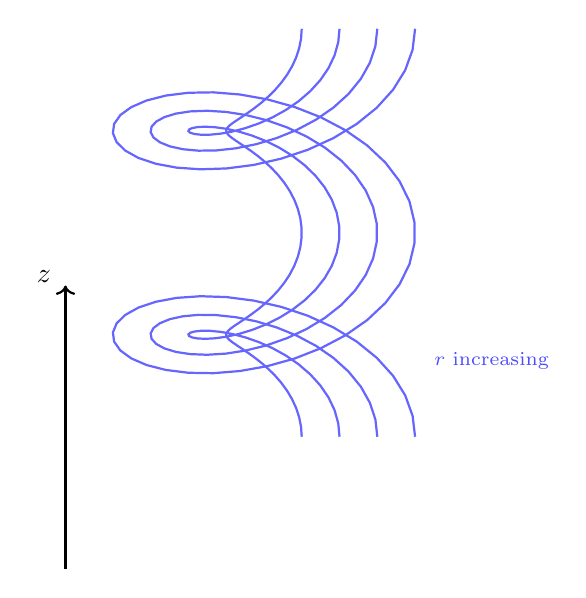
\begin{tikzpicture}[scale=0.6]
    \foreach \r in {0.8, 1.6, 2.4, 3.2} {
        \draw[blue!60, thick, domain=0:720, samples=70, variable=\t]
            plot ({\r*cos(\t)}, {0.55*\r*sin(\t) + 0.012*\t});
    }
    \draw[->, thick] (-4.2, -2.8) -- (-4.2, 3.2);
    \node[left] at (-4.3, 3.4) {$z$};
    \node[right, blue!70, font=\scriptsize] at (3.4, 1.6) {$r$ increasing};
\end{tikzpicture}
\caption{Illustrative helical field lines. The local pitch varies with the ratio $B_z/B_\theta$ according to Eq.~\eqref{eq:pitch}.}
\label{fig:fieldlines}
\end{figure}

\section{Magnetization Regime}
\label{sec:magnetization}

The proposed baseline operating point uses argon at 10~mTorr with an axial field of 100~G. Whether a species is magnetized is set by its Hall parameter, the ratio of cyclotron frequency to collision frequency with the neutral background:
\begin{equation}
H_s = \frac{\omega_{c,s}}{\nu_{s,n}} = \frac{q_s B / m_s}{n_n \sigma_{s,n} \bar{v}_{s}},
\label{eq:hall}
\end{equation}
where $s \in \{e, i\}$ and $n_n$ is the neutral density set by the fill pressure. Species with $H_s \gg 1$ are magnetized; species with $H_s \lesssim 1$ are not. For argon at 10~mTorr ($n_n \approx 3\times10^{20}\ \mathrm{m}^{-3}$ at room temperature), electrons satisfy $H_e \gg 1$ already at tens of gauss, since $\omega_{ce}$ is large and electron-neutral collisionality is comparatively low. Ions, being $\sim\!7\times10^4$ times heavier, have a correspondingly smaller $\omega_{ci}$ at fixed $B$; at 100~G, $H_i \sim 0.1$--$0.3$ using representative ion-neutral cross sections $\sigma_{in} \sim 10^{-18}\ \mathrm{m}^2$, so ions remain unmagnetized while electrons are strongly magnetized. Raising $B$ toward $\sim$1~kG increases $H_i$ to order unity, marking the onset of ion magnetization and providing a clear, quantitatively grounded regime boundary that can be explored experimentally by scanning $B$ at fixed pressure.

Figure~\ref{fig:regime} maps these boundaries across the accessible $B$--$p$ space. The baseline operating point (A) sits well inside the electron-magnetized helicon band, and the proposed field scan traverses continuously to the onset of ion magnetization (B, where $H_i = 1$ at approximately 530~G for the parameters above) and beyond: the device can move from electron-only magnetization to combined electron--ion magnetization without changing gas conditions.

\begin{figure}[htbp]
\centering
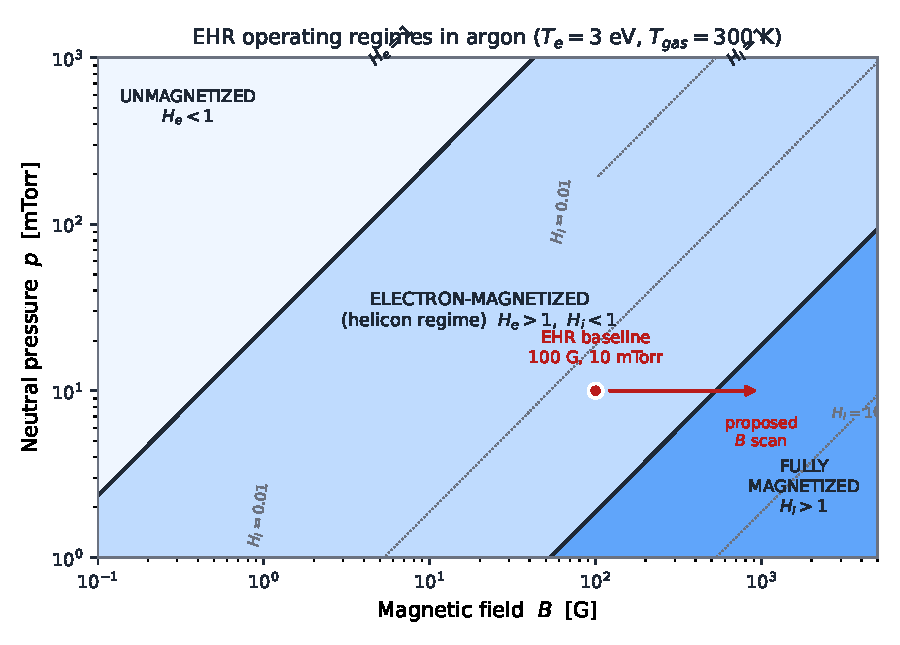
\includegraphics[width=0.92\textwidth]{figures/ehr-regime-map.pdf}
\caption{Operating-regime map for argon in the $B$--$p$ plane, with Hall-parameter contours from Eq.~\eqref{eq:hall}. Point A is the baseline operating point; point B marks the onset of ion magnetization ($H_i=1$) reached by the proposed field scan at fixed pressure. Regime boundaries depend on the assumed collision cross sections and characteristic particle velocities ($T_e = 3$~eV, $T_{\mathrm{gas}} = 300$~K, $\sigma_{en} = 2\times10^{-20}$~m$^2$, $\sigma_{in} = 10^{-18}$~m$^2$) and should be interpreted as order-of-magnitude estimates.}
\label{fig:regime}
\end{figure}

\section{Resonance-Matched Power Coupling}

Efficient power deposition is achieved by coupling to the helicon mode, whose resonance condition links drive frequency, wavenumber, plasma density, and magnetic field through the helicon dispersion relation \cite{chenarnush1997,boswell1984,chen2015}. For the $m=1$ mode in the low-frequency (whistler) limit, this relation takes the form
\begin{equation}
\omega = \frac{k\, k_\perp\, B_0}{\mu_0 n_e e}\,,
\label{eq:dispersion}
\end{equation}
where $k$ is the axial wavenumber set by the antenna, $k_\perp$ is the radial eigenvalue fixed by the boundary condition at the chamber wall, and $n_e$ is the electron density. Equation~\eqref{eq:dispersion} defines a resonance surface in $(\omega, k, B_0, n_e)$ space: at fixed antenna frequency and geometry, sweeping $B_0$ or allowing $n_e$ to respond self-consistently moves the operating point across this surface, producing the density peak identified as Prediction 2 in Section~\ref{sec:validation}.

\section{Governing Equations}

Single-particle motion obeys the Lorentz force,
\begin{equation}
m_s \frac{d\mathbf{v}}{dt} = q_s\left(\mathbf{E} + \mathbf{v}\times\mathbf{B}\right) + \mathbf{F}_{\mathrm{coll}},
\label{eq:lorentz}
\end{equation}
with $\mathbf{B} = \mathbf{B}(r) + \tilde{\mathbf{B}}$ given by Eqs.~\eqref{eq:bfield}--\eqref{eq:helicon} and $\mathbf{F}_{\mathrm{coll}}$ the Monte-Carlo collision force with the neutral background. The corresponding fluid momentum equation is
\begin{equation}
m_s n_s \left(\frac{\partial \mathbf{u}_s}{\partial t} + \mathbf{u}_s\cdot\nabla \mathbf{u}_s\right) = q_s n_s\left(\mathbf{E} + \mathbf{u}_s\times\mathbf{B}\right) - \nabla p_s + \mathbf{F}_{\mathrm{ac}},
\label{eq:fluid}
\end{equation}
where $\mathbf{F}_{\mathrm{ac}}$ is an additional body-force term representing momentum transfer from the acoustically modulated neutral background, and is nonzero only where the standing-wave drive of Section~\ref{sec:acoustic} is active.

\section{Acoustic Standing-Wave Modulation}
\label{sec:acoustic}

Acoustic standing waves are proposed as an independent control channel acting on the neutral gas (Fig.~\ref{fig:modes}). At 10~mTorr, acoustic radiation forces are weak and damping is strong. The EHR is therefore positioned as a research platform to explore neutral-to-plasma coupling at the centimeter scale. Sustaining well-defined standing waves would require resonant drive or operation at moderately higher pressure.

\begin{figure}[htbp]
\centering
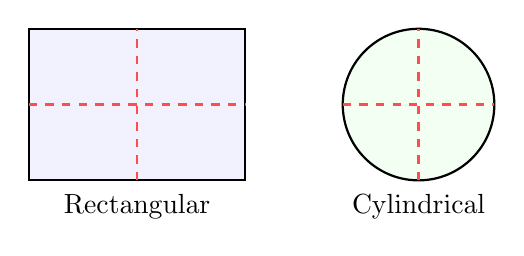
\begin{tikzpicture}[scale=0.55]
    \draw[thick, fill=blue!5] (0,0) rectangle (5,3.5);
    \draw[thick, dashed, red!70] (0,1.75) -- (5,1.75);
    \draw[thick, dashed, red!70] (2.5,0) -- (2.5,3.5);
    \node at (2.5,-0.6) {Rectangular};

    \draw[thick, fill=green!5] (9,1.75) circle (1.75);
    \draw[thick, dashed, red!70] (9,0) -- (9,3.5);
    \draw[thick, dashed, red!70] (7.25,1.75) -- (10.75,1.75);
    \node at (9,-0.6) {Cylindrical};
\end{tikzpicture}
\caption{Illustrative acoustic standing-wave modes. Red lines indicate pressure nodes.}
\label{fig:modes}
\end{figure}

\section{Sanity-Check Scaling Estimates}
\label{sec:scaling}

The following order-of-magnitude estimates, all at the baseline operating point (argon, 10~mTorr, 100~G, $T_e = 3$~eV, $T_{\mathrm{gas}} = 300$~K), make the assumptions behind the proposed architecture explicit and auditable.

\begin{itemize}
    \item \textbf{Neutral density and mean free path.} $n_n = p / k_B T_{\mathrm{gas}} \approx 3.2\times10^{20}\ \mathrm{m}^{-3}$. With $\sigma_{nn} \sim 10^{-18}\ \mathrm{m}^2$, the neutral--neutral mean free path is $\lambda_n = (\sqrt{2}\, n_n \sigma_{nn})^{-1} \approx 2$~mm, giving a Knudsen number of order $10^{-2}$ for a 10-cm-scale chamber. The gas is only marginally in the continuum regime: classical acoustics applies, but damping is strong and textbook standing-wave behavior cannot be assumed.
    \item \textbf{Electron magnetization.} With $\sigma_{en} \approx 2\times10^{-20}\ \mathrm{m}^2$ at a few eV, Eq.~\eqref{eq:hall} gives $H_e \approx 240$ at 100~G: electrons are strongly magnetized throughout the proposed operating range.
    \item \textbf{Ion magnetization.} With $\sigma_{in} \approx 10^{-18}\ \mathrm{m}^2$, $H_i \approx 0.19$ at 100~G, crossing unity at $\approx 530$~G and reaching $\approx 1.9$ at 1~kG --- the basis for the regime boundary of Fig.~\ref{fig:regime}.
    \item \textbf{Acoustic density modulation.} At 10~mTorr the background pressure is $P_0 \approx 1.33$~Pa. For acoustic pressure amplitudes $\Delta P = 0.01$--$0.1$~Pa, the expected neutral-density perturbation is $\Delta n_n / n_n \approx \Delta P / P_0 \approx 0.8$--$8\%$. The ability to achieve such amplitudes at 10~mTorr remains an experimental question and constitutes the primary uncertainty of the proposed acoustic-control channel.
    \item \textbf{Helicon resonance range.} For a chamber radius $R = 0.1$~m ($k_\perp \approx 3.83/R \approx 38\ \mathrm{rad/m}$), an antenna wavenumber $k \approx 20\ \mathrm{rad/m}$, and $B_0 = 100$~G, Eq.~\eqref{eq:dispersion} places the resonance at $n_e \approx 4.5\times10^{17}\ \mathrm{m}^{-3}$ for a 13.56~MHz drive --- squarely within the density range of conventional helicon sources.
\end{itemize}

These estimates use representative cross sections and thermal velocities; the resulting numbers should be read as order-of-magnitude guides rather than predictions, and the sensitivity of each to the assumed parameters is itself a target for the validation program of Section~\ref{sec:validation}.

\section{Applications}

The architecture targets improved across-wafer uniformity in processes such as tungsten metallization and SiC etching. Magnetic field management near the wafer remains important to minimize non-uniformity and charging damage. The device is also proposed as a flexible platform for fundamental studies of helicon-acoustic coupling and dusty plasma dynamics under controlled conditions.

\section{Proposed Experimental Validation}
\label{sec:validation}

Four falsifiable predictions are defined at the baseline operating point of Section~\ref{sec:magnetization}:

\begin{enumerate}
    \item The $m=1$ helicon mode can be directly measured with a phase-resolved B-dot probe array \cite{hutchinson} and shown to satisfy the helicon dispersion relation.
    \item Scanning the drive frequency or magnetic field strength through the helicon resonance condition produces a measurable peak in plasma density.
    \item Acoustic standing-wave drive imprints measurable centimeter-scale periodic modulation on both the neutral gas density and the plasma density. Given the amplitude estimates of Section~\ref{sec:scaling}, a reproducible modulation of $\Delta n/n \gtrsim 0.5$--$1\%$ synchronized with the acoustic drive would suffice to establish the coupling channel.
    \item Scanning the field-line pitch of Eq.~\eqref{eq:pitch} via the coil-current ratio, at constant $|B|$ and RF power, produces measurable changes in the coupled power and plasma density profile.
\end{enumerate}

Failure of the third prediction would indicate that acoustic modulation does not couple effectively to the plasma under the proposed conditions. Failure of the fourth --- no pitch-dependent effects at constant $|B|$ and power --- would indicate that the tunable helical geometry does not provide meaningful additional control.

\section{Dusty Plasma Dynamics and Ion Drag}

When micron-sized particles are introduced into the plasma, they acquire substantial negative charge and experience several forces. The ion drag force, arising from both direct ion collection and Coulomb scattering, is often dominant in low-pressure discharges and governs dust transport, void formation, and dust-acoustic waves \cite{goree2020}.

The EHR architecture offers experimental handles that are not readily available in conventional dusty plasma devices. The tunable helical magnetic field allows controlled modification of ion flow patterns through changes in field-line pitch at constant $|B|$. Acoustic standing-wave modulation provides an external means to influence the neutral gas background, which, through ion-neutral collisions, can affect local ion trajectories and the resulting ion drag.

\section{Plasma Crystal Formation}

Micron-sized dust particles in a plasma acquire large negative charges and interact via a screened (Yukawa) repulsive potential. When the coupling parameter
\begin{equation}
\Gamma = \frac{Q_d^2}{4\pi\epsilon_0 a k_B T_d} \exp\left( -\frac{a}{\lambda_D} \right)
\end{equation}
--- where $Q_d$ is the dust charge, $a$ the interparticle spacing, $T_d$ the dust kinetic temperature, and $\lambda_D$ the Debye screening length --- becomes sufficiently large, the particles can self-organize into ordered crystalline structures known as plasma crystals. In two-dimensional laboratory systems, strong ordering is typically observed for $\Gamma \gtrsim 130$--$150$ \cite{melzer1996}. In three-dimensional Yukawa systems, the melting transition generally occurs at higher values, typically $\Gamma \gtrsim 170$--$200$ for moderate screening, with the exact threshold depending on the screening parameter $\kappa = a / \lambda_D$ \cite{hamaguchi1997}.

The EHR architecture offers experimental capabilities well suited to studying these strongly coupled regimes. The tunable helical magnetic field enables controlled modification of ion flow and ion wake structures, while acoustic modulation provides a means to externally influence dust kinetic temperature or drive the system across the crystallization threshold.

\section{Magnetized Ion Wake Dynamics}

In a flowing dusty plasma, ions streaming past negatively charged dust particles create localized regions of positive space charge known as ion wakes. These wakes make the effective dust–dust interaction non-reciprocal. A representative form of the electrostatic potential combines the screened Coulomb contribution with an oscillatory wake term:
\begin{equation}
\phi(r_\perp, z) \approx \frac{Q_d}{4\pi\epsilon_0} \left[
\frac{\exp(-r/\lambda_D)}{r}
+ A \frac{\exp(-|z|/\ell_w)}{r} \sin(k_z |z|)
\right],
\label{eq:wake}
\end{equation}
where $r = \sqrt{r_\perp^2 + z^2}$, $z < 0$ is the downstream direction, $A$ is a dimensionless wake amplitude, $\ell_w$ is the wake decay length, and $k_z$ is the wake wavenumber set by the ion flow speed.

When ions become magnetized, their trajectories transition from straight lines to helical motion. This modifies the wake structure, making the screening anisotropic and altering both the amplitude and spatial form of the wake-mediated interaction. The EHR architecture is designed to allow controlled investigation of this transition. At the baseline field of 100~G, ions remain unmagnetized. As the field is increased toward $\sim$1~kG, ions begin to magnetize. The tunable helical geometry further enables variation of the angle between $\mathbf{B}$ and the ion flow at fixed field strength.

\section{Discussion}

The EHR combines established physical elements — helical magnetic fields, helicon wave coupling, and acoustic modulation — into a single device with two programmable control variables. The primary technical challenges include efficient acoustic coupling at low pressure, thermal management of transducers, and careful management of magnetic fields near the wafer. Quantitative modeling of expected performance gains remains a subject for future work.

\section{Conclusion}

The Electromagnetic Helix Reactor proposes an integrated architecture in which a tunable helical magnetic field, helicon drive, and acoustic modulation operate within a physically consistent regime. A four-prediction experimental program provides clear criteria for validation or falsification. If successful, the concept offers a path toward improved spatial control in low-temperature plasma processing and a versatile platform for fundamental studies of wave-driven and dusty plasmas under controlled ion flow conditions.

\section*{Code Availability}
An interactive, browser-based reduced-physics simulator of the EHR concept --- implementing the helical field models, Boris-integrated electron dynamics with Monte-Carlo collisions, helicon coupling models, synthetic diagnostics, and the dusty-plasma module discussed here --- is openly available at \url{https://github.com/ZachBach/ElectromagneticHelixReactor}.

\section*{Authorship Statement}
This work was developed and authored solely by Zachary Auerbach with no external funding or collaborators.

\begin{thebibliography}{99}
\bibitem{lieberman} M.~A. Lieberman and A.~J. Lichtenberg, \textit{Principles of Plasma Discharges and Materials Processing}, 2nd ed., Wiley, 2005.
\bibitem{chabert} P.~Chabert and N.~Braithwaite, \textit{Physics of Radio-Frequency Plasmas}, Cambridge University Press, 2011.
\bibitem{oehrlein2018} G.~S. Oehrlein and S.~Hamaguchi, ``Foundations of low-temperature plasma enhanced materials synthesis and etching,'' \textit{Plasma Sources Sci. Technol.} \textbf{27}, 023001 (2018).
\bibitem{boswell1984} R.~W. Boswell, ``Very efficient plasma generation by whistler waves near the lower hybrid frequency,'' \textit{Plasma Phys. Control. Fusion} \textbf{26}, 1147 (1984).
\bibitem{chen2015} F.~F. Chen, ``Helicon discharges and sources: a review,'' \textit{Plasma Sources Sci. Technol.} \textbf{24}, 014001 (2015).
\bibitem{chenarnush1997} F.~F. Chen and D.~Arnush, ``Generalized theory of helicon waves. I. Normal modes,'' \textit{Phys. Plasmas} \textbf{4}, 3411 (1997).
\bibitem{asmussen1989} J.~Asmussen, ``Electron cyclotron resonance microwave discharges for etching and thin-film deposition,'' \textit{J. Vac. Sci. Technol. A} \textbf{7}, 883 (1989).
\bibitem{gorkov1962} L.~P. Gor'kov, ``On the forces acting on a small particle in an acoustical field in an ideal fluid,'' \textit{Sov. Phys. Dokl.} \textbf{6}, 773 (1962).
\bibitem{bruus2012} H.~Bruus, ``Acoustofluidics 7: The acoustic radiation force on small particles,'' \textit{Lab Chip} \textbf{12}, 1014 (2012).
\bibitem{goree2020} J.~Goree \textit{et al.}, ``Correlation and spectrum of dust acoustic waves in a radio-frequency plasma using PK-4 on the International Space Station,'' \textit{Phys. Plasmas} \textbf{27}, 123701 (2020).
\bibitem{hutchinson} I.~H. Hutchinson, \textit{Principles of Plasma Diagnostics}, 2nd ed., Cambridge University Press, 2002.
\bibitem{freidberg} J.~P. Freidberg, \textit{Ideal MHD}, Cambridge University Press, 2014.
\bibitem{melzer1996} A.~Melzer, A.~Homann, and A.~Piel, ``Experimental investigation of the melting transition of the plasma crystal,'' \textit{Phys. Rev. E} \textbf{53}, 2757 (1996).
\bibitem{hamaguchi1997} S.~Hamaguchi, R.~T. Farouki, and D.~H.~E. Dubin, ``Triple point of Yukawa systems,'' \textit{Phys. Rev. E} \textbf{56}, 4671 (1997).
\end{thebibliography}

\end{document}
